\chapter{Neural Networks}


\section{Model Representation}
\begin{itemize}
    \item Neural networks were developed as simulating neurons or networks of neurons in the brain.
    \item Neurons are basically computational units that take inputs (dendrites) as electrical inputs (called ``spikes'') that are channeled to outputs (axons).
    \begin{figure}[H]
        \centering
        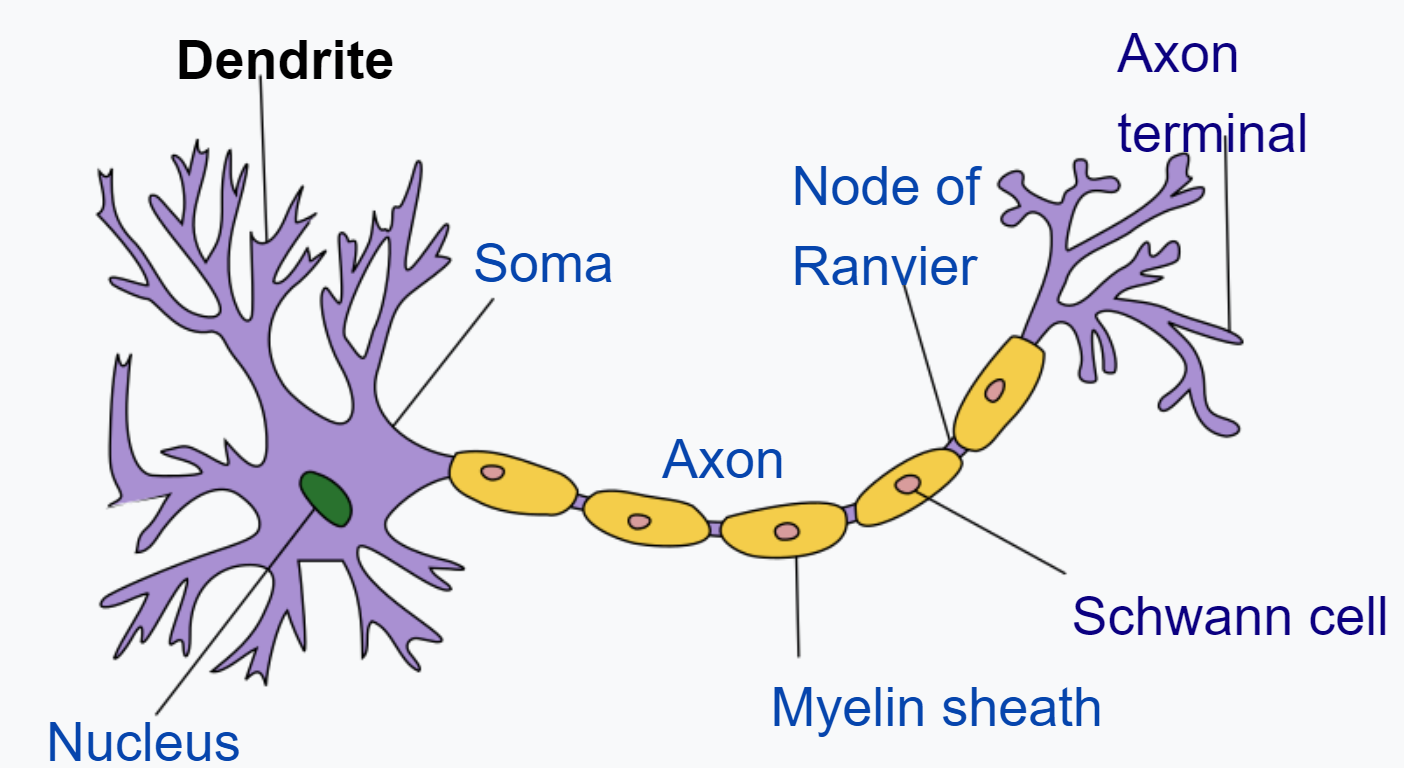
\includegraphics[width=2.8in]{./images/neuron.png}
        \caption{Neuron in the brain}
    \end{figure}
    
    \item Visually, a simple forward propagation looks like:
    \begin{figure}[H]
        \centering
        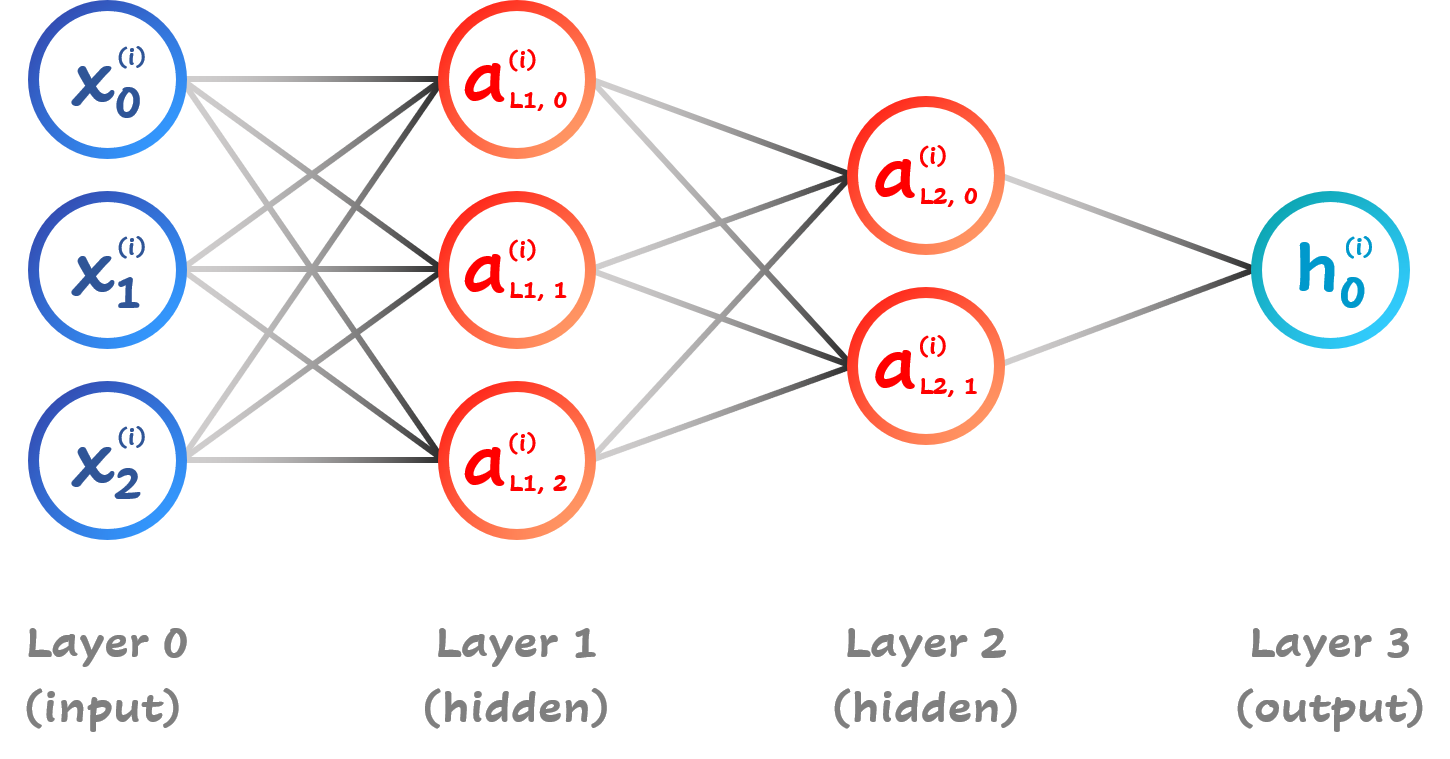
\includegraphics[width=3.8in]{./images/neuron_networks_architecture.png}
        \caption{Neural networks architecture}
    \end{figure}

    \begin{figure}[H]
        \centering
        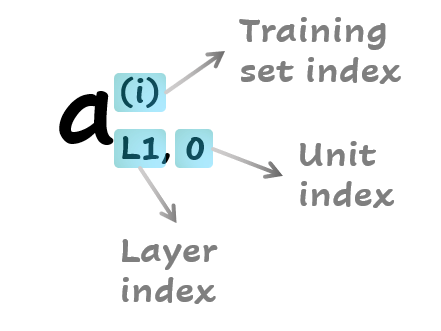
\includegraphics[width=2.1in]{./images/super_subscript.png}
        \caption{The convention of the superscript and subscript in neural networks}
    \end{figure}
    
    \item Neural networks can also do multiclass classification
    \begin{figure}[H]
        \centering
        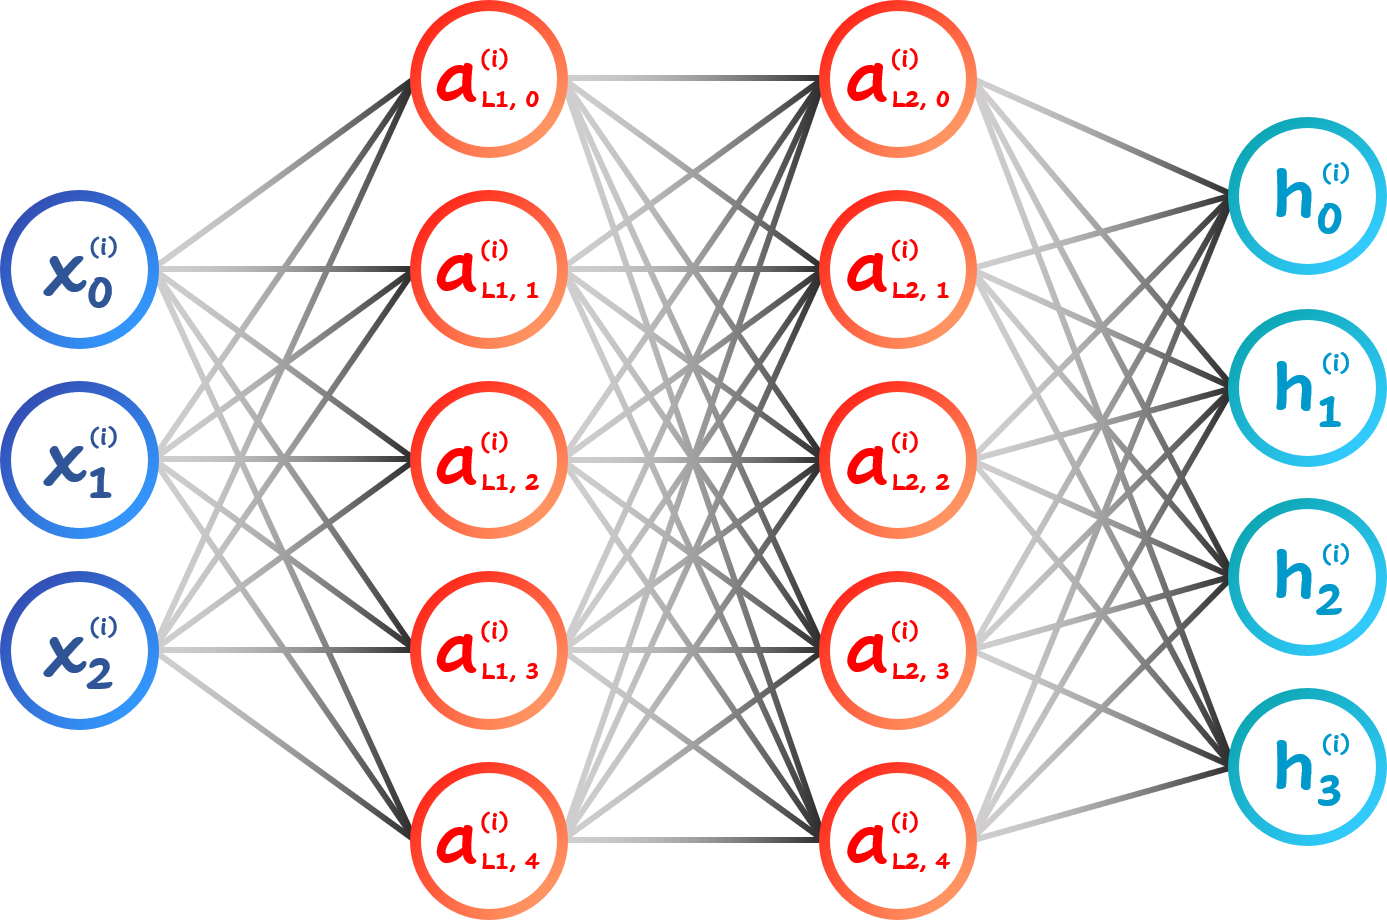
\includegraphics[width=3.8in]{./images/multiClassClassification.png}
        \caption{neural network for multi-class classification}
    \end{figure}

    \begin{equation}
        \mathbf{h} \approx \left\{ \begin{array}{l}

        \left[ \begin{matrix} 1 & 0 & 0 & 0 \end{matrix} \right]^T \text{, for pedestrian}\\
        \left[ \begin{matrix} 0 & 1 & 0 & 0 \end{matrix} \right]^T \text{, for car}\\
        \left[ \begin{matrix} 0 & 0 & 1 & 0 \end{matrix} \right]^T \text{, for motocycle}\\
        \left[ \begin{matrix} 0 & 0 & 0 & 1 \end{matrix} \right]^T \text{, for truck}\\

        \end{array}\right.
    \end{equation}

    \item In neural networks, the logistic function is sometimes called a \textbf{activation} function. In this situation, parameters are sometimes called \textbf{weights}.
    The values for each of the activation nodes is obtained as follows:
    \begin{equation}
        \begin{aligned}
            a_{L1,0} &= g(\theta_{L1, 00}x_0 + \theta_{L1, 01}x_1 + \theta_{L1, 02}x_2 + \theta_{L1, 03}x_3) &= g(z_{L1, 0})\\
            a_{L1,1} &= g(\theta_{L1, 10}x_0 + \theta_{L1, 11}x_1 + \theta_{L1, 12}x_2 + \theta_{L1, 13}x_3) &= g(z_{L1, 0})\\
            a_{L1,2} &= g(\theta_{L1, 20}x_0 + \theta_{L1, 21}x_1 + \theta_{L1, 22}x_2 + \theta_{L1, 23}x_3) &= g(z_{L1, 0})\\
        \end{aligned}
    \end{equation}

    Where $a_{Lj,i}$ means the activation of \textbf{unit} $i$ in layer $j$, and $\Theta_{Lj}$ means a mapping matrix of weights from layer $j-1$ to layer $j$.
    If there are $s_j$ units in layer $j$ and $s_{j-1}$ units in layer $j-1$, then.
    \begin{equation}
        \Theta_{Lj} =
        \left[
        \begin{matrix}
            \theta_{Lj, 00}     & \theta_{Lj, 01}     & \dots   & \theta_{Lj, 0{s_{j-1}}}     \\
            \theta_{Lj, 10}     & \theta_{Lj, 11}     & \dots   & \theta_{Lj, 1{s_{j-1}}}     \\
            \vdots              & \vdots              & \ddots  & \vdots                      \\
            \theta_{Lj, {s_j}0} & \theta_{Lj, {s_j}1} & \dots   & \theta_{Lj, {s_j}{s_{j-1}}} \\
        \end{matrix}
        \right]_{{(s_j+1)} \times {(s_{j-1}+1)}}
    \end{equation}
\end{itemize}

    
\section{Simplified Expressions}
\begin{itemize}
    \item The neural network looks too fancy. Let's try to make it simpler but more boring. The network could be expressed like:

    \begin{equation}
        \left[\begin{matrix} x^{(i)}_0 \\ x^{(i)}_1 \\ x^{(i)}_2 \end{matrix}\right]_{3 \times 1} \xRightarrow{[\Theta_{L1}]_{5 \times 3}}
        \left[\begin{matrix} a^{(i)}_{L1, 0} \\ a^{(i)}_{L1, 1} \\ a^{(i)}_{L1, 2} \\ a^{(i)}_{L1, 3} \\ a^{(i)}_{L1, 4} \end{matrix}\right]_{5 \times 1} \xRightarrow{[\Theta_{L2}]_{5 \times 5}}
        \left[\begin{matrix} a^{(i)}_{L2, 0} \\ a^{(i)}_{L2, 1} \\ a^{(i)}_{L2, 2} \\ a^{(i)}_{L2, 3} \\ a^{(i)}_{L2, 4} \end{matrix}\right]_{5 \times 1} \xRightarrow{[\Theta_{L3}]_{4 \times 5}}
        \left[\begin{matrix} h_0 \\ h_1 \\ h_2 \\ h_3 \end{matrix}\right]_{4 \times 1}
    \end{equation}

    \item Or in a vectorized form:
    \begin{equation}
        \mathbf{x}^{(i)} \xRightarrow{\Theta_{L1}}
        \mathbf{a}^{(i)}_{L1} \xRightarrow{\Theta_{L2}}
        \mathbf{a}^{(i)}_{L2} \xRightarrow{\Theta_{L3}}
        \mathbf{h}^{(i)}
    \end{equation}

    \item Actually, only three linear algebra equations are needed for this neural network
    \begin{equation}
        \begin{aligned}
            \mathbf{a}^{(i)}_{L1} &= g(\Theta_{L1} \times \mathbf{x}^{(i)})\\
            \mathbf{a}^{(i)}_{L2} &= g(\Theta_{L2} \times \mathbf{a}^{(i)}_{L1})\\
            \mathbf{h}^{(i)}      &= g(\Theta_{L3} \times \mathbf{a}^{(i)}_{L2})\\
        \end{aligned}
    \end{equation}
\end{itemize}

\section{Cost Function}
\begin{itemize}
    \item The cost function of a neural network with $m$ data sets, $K$ classifications and $L$ layers
    \begin{equation}
        J(\theta) = \frac{-1}{m}\sum_{i=1}^{m}\sum_{k=1}^{K}\left[ y^{(i)}_k \log\left(h^{(i)}_k\right) + \left(1 - y^{(i)}_k \right) \log\left(1 - h^{(i)}_k\right) \right] + \frac{\lambda}{2m}\sum_{l=1}^{L}||\Theta_{Ll}||_2^2
    \end{equation}
    Where $||\Theta_{Ll}||_2$ means \href{https://mathworld.wolfram.com/FrobeniusNorm.html}{Frobenius norm} of the matrix $\Theta_{Ll}$ 
\end{itemize}


\section{Backpropagation Algorithm}
\begin{itemize}
    \item Consider a simple neural network with only one data set
    \begin{figure}[H]
        \centering
        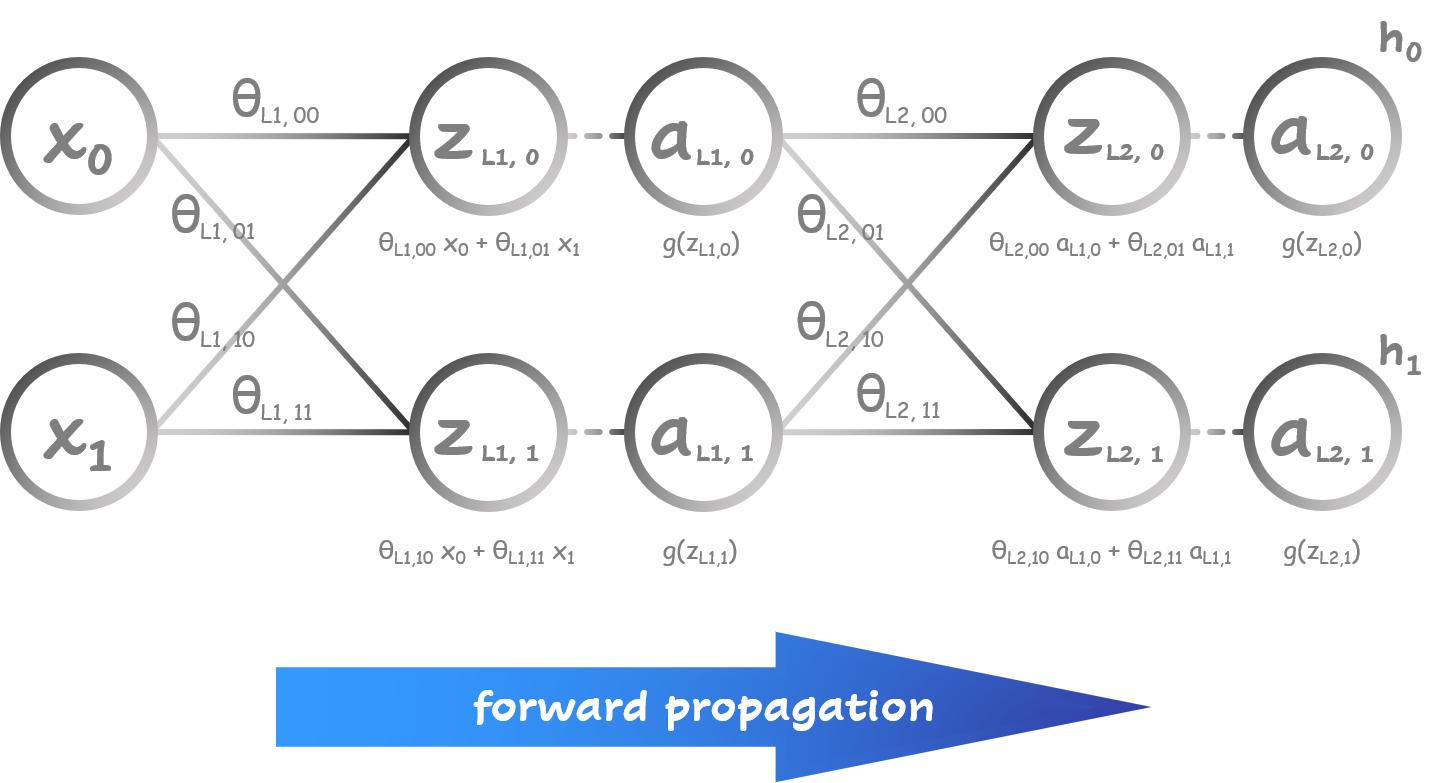
\includegraphics[width=4.8in]{./images/neural_network_forward.png}
        \caption{A simple neural network}
    \end{figure}
    
    The cost function would be
    \begin{equation}
        J(\theta) = \left[ 
                        y_0 \log\left(h_0\right) + \left(1 - y_0 \right) \log\left(1 - h_0\right) + 
                        y_1 \log\left(h_1\right) + \left(1 - y_1 \right) \log\left(1 - h_1\right) 
                    \right]
    \end{equation}

    And the gradient descent iteration would be:
    \begin{equation}
        \theta_{l, ij} \coloneqq \theta_{l, ij} - \alpha\frac{\partial J(\theta)}{\partial \theta_{l, ij}} 
    \end{equation}
    
    To compute the gradient descent for $\theta_{l, ij}$, it's needed to find out the regulation of $\frac{\partial J}{\partial \theta_{l,ij}}$.
    First, try to do the partial derivatives at the second layer.
    
    \begin{equation}
        \frac{\partial J}{\partial \theta_{L2,00}} = \frac{\partial J}{\partial a_{L2,0}}\frac{\partial a_{L2,0}}{\partial z_{L2,0}}\frac{\partial z_{L2,0}}{\partial \theta_{L2,00}} = \frac{\partial J}{\partial a_{L2,0}} g'(z_{L2,0}) a_{L1,0}
    \end{equation}
    \begin{equation}
        \frac{\partial J}{\partial \theta_{L2,01}} = \frac{\partial J}{\partial a_{L2,0}}\frac{\partial a_{L2,0}}{\partial z_{L2,0}}\frac{\partial z_{L2,0}}{\partial \theta_{L2,01}} = \frac{\partial J}{\partial a_{L2,0}} g'(z_{L2,0}) a_{L1,1}
    \end{equation}
    \begin{equation}
        \frac{\partial J}{\partial \theta_{L2,10}} = \frac{\partial J}{\partial a_{L2,1}}\frac{\partial a_{L2,1}}{\partial z_{L2,1}}\frac{\partial z_{L2,1}}{\partial \theta_{L2,10}} = \frac{\partial J}{\partial a_{L2,1}} g'(z_{L2,1}) a_{L1,0}
    \end{equation}
    \begin{equation}
        \frac{\partial J}{\partial \theta_{L2,11}} = \frac{\partial J}{\partial a_{L2,1}}\frac{\partial a_{L2,1}}{\partial z_{L2,1}}\frac{\partial z_{L2,1}}{\partial \theta_{L2,11}} = \frac{\partial J}{\partial a_{L2,1}} g'(z_{L2,1}) a_{L1,1}
    \end{equation}
    
    Then, try to do the partial derivatives at the first layer.
    \begin{equation}\label{eqn:partialDerivative}
        \begin{aligned}
            \frac{\partial J}{\partial \theta_{L1,00}} &= \left({ \frac{\partial J}{\partial a_{L2,0}}\frac{\partial a_{L2,0}}{\partial z_{L2,0}}\frac{\partial z_{L2,0}}{\partial a_{L1,0}} + \frac{\partial J}{\partial a_{L2,1}}\frac{\partial a_{L2,1}}{\partial z_{L2,1}}\frac{\partial z_{L2,1}}{\partial a_{L1,0}} }\right) \frac{\partial a_{L1,0}}{\partial z_{L1,0}}\frac{\partial z_{L1,0}}{\partial \theta_{L1,00}}\\
                                                        &= \left({ \frac{\partial J}{\partial a_{L2,0}} g'(z_{L2,0}) \theta_{L2,00} + \frac{\partial J}{\partial a_{L2,1}} g'(z_{L2,1}) \theta_{L2,10}} \right) g'(z_{L1,0}) x_0 \\
                                                        &= \frac{\partial J}{\partial a_{L1,0}} g'(z_{L1,0}) x_0 \\
        \end{aligned}
    \end{equation}
    
    So the others would be like
    \begin{equation}
        \frac{\partial J}{\partial \theta_{L1,01}} = \frac{\partial J}{\partial a_{L1,0}} g'(z_{L1,0}) x_1
    \end{equation}
    \begin{equation}
        \frac{\partial J}{\partial \theta_{L1,10}} = \frac{\partial J}{\partial a_{L1,1}} g'(z_{L1,1}) x_0
    \end{equation}
    \begin{equation}
        \frac{\partial J}{\partial \theta_{L1,11}} = \frac{\partial J}{\partial a_{L1,1}} g'(z_{L1,1}) x_1
    \end{equation}
    
    It can be seen that $\frac{\partial{J}}{\partial{a_{l,i}}}$ are necessary for $\frac{\partial{J}}{\partial{\theta_{l,ij}}}$.
    However, if using a forward propagation to do the gradient descent process,
    it would be unavailable for $\frac{\partial{J}}{\partial{a_{l,i}}}$ at a previous layer because of the dependency in a neural network.
    To solve this inconvenience, backpropagation should be adopted.
    
    That is to say the training processes of a neural network containing 
    one forward process to get the values of each activations ($a_{l,i}$) and 
    one backpropagation process to get the values of derivatives corresponded to each activations ($\frac{\partial{J}}{\partial{a_{L,i}}}$).
    Then the values derived from the backpropagation are necessary for the gradient descent process.
    
    Observe equation \ref{eqn:partialDerivative}, there is a regulation of $\frac{\partial{J}}{\partial{a_{l,i}}}$ can be found. 
    The regulation can be seen as actions of the backpropagation process in Figure \ref{fig:backpropagation}.
    
    \begin{figure}[H] \label{fig:backpropagation}
        \centering
        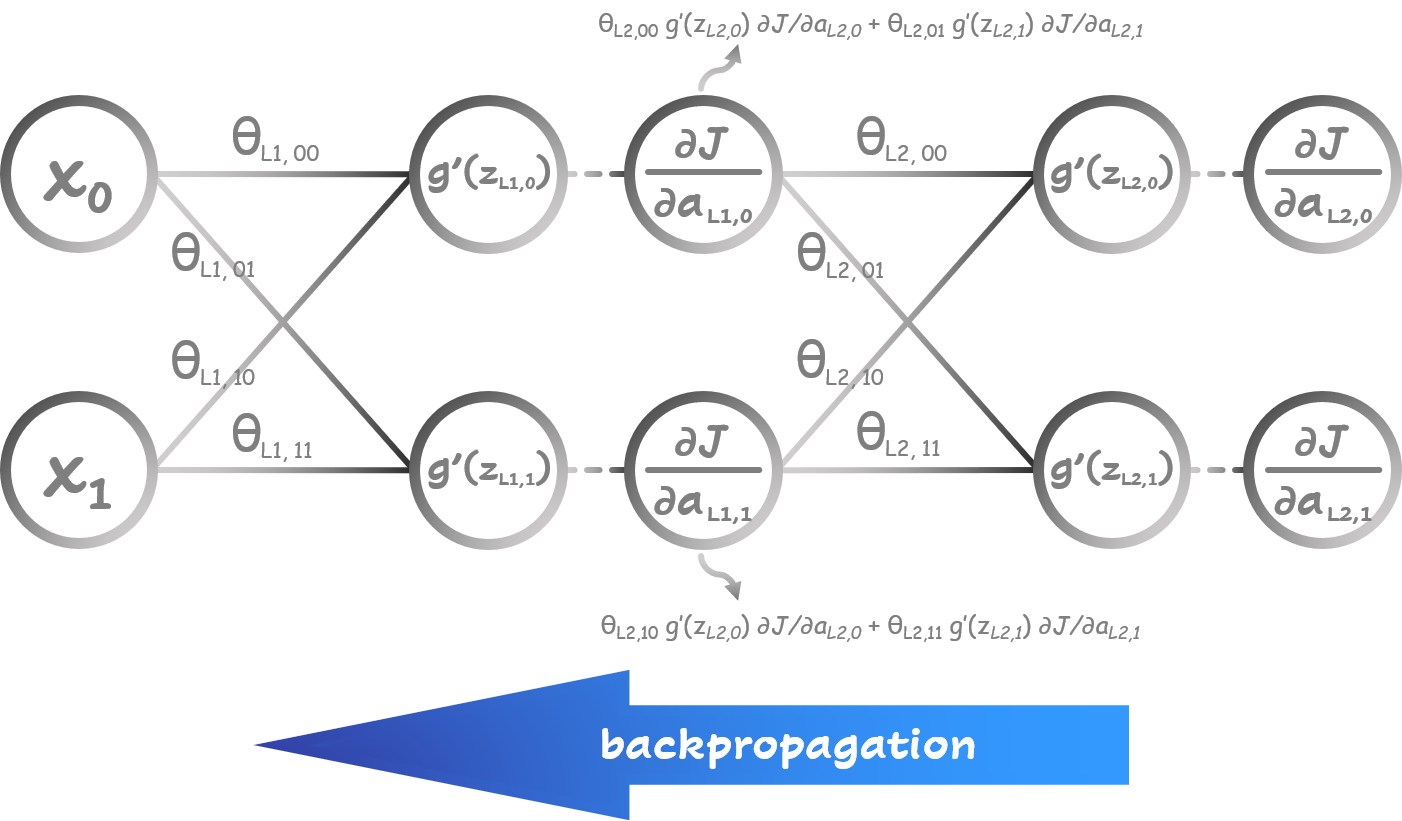
\includegraphics[width=4.8in]{./images/neural_network_back.png}
        \caption{The backpropagation in a neural network}
    \end{figure}
    
    Once the backpropagation process was completed, the partial derivatives of each weight ($\frac{\partial J}{\partial \theta_{l,ij}}$) 
    can computed which is shown as figure \ref{fig:gradientDescentNN} and equation \ref{eqn:gradientDescentNN}
    
    \begin{figure}[H] \label{fig:gradientDescentNN}
        \centering
        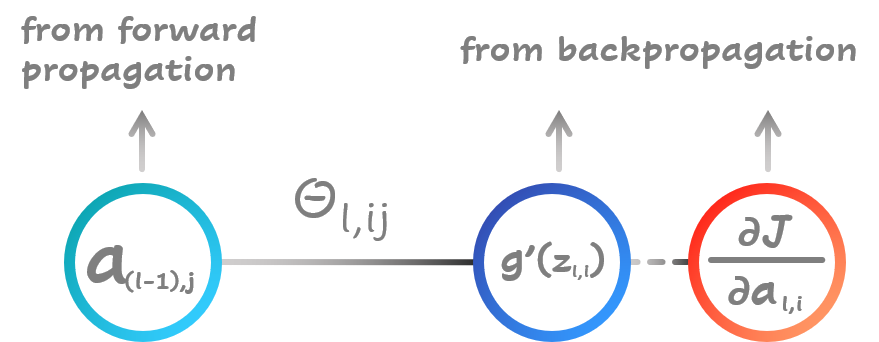
\includegraphics[width=3.6in]{./images/gradient_descent_neural_network.png}
        \caption{The backpropagation in a neural network}
    \end{figure}
    
    \begin{equation} \label{eqn:gradientDescentNN}
        \frac{\partial J}{\partial \theta_{l,ij}} = \color{RedOrange} \frac{\partial J}{\partial a_{l,i}} \color{blue} g'(z_{l,i}) \color{cyan} a_{(l-1),j} \color{black}
    \end{equation}
\end{itemize}
    
    
\section{Non-linear Classification Example}
\begin{itemize}
    \item Logical functions in figure \ref{fig:logicGates} would be examples to show how neural networks really work.
    \begin{figure}[H]\label{fig:logicGates}
        \centering
        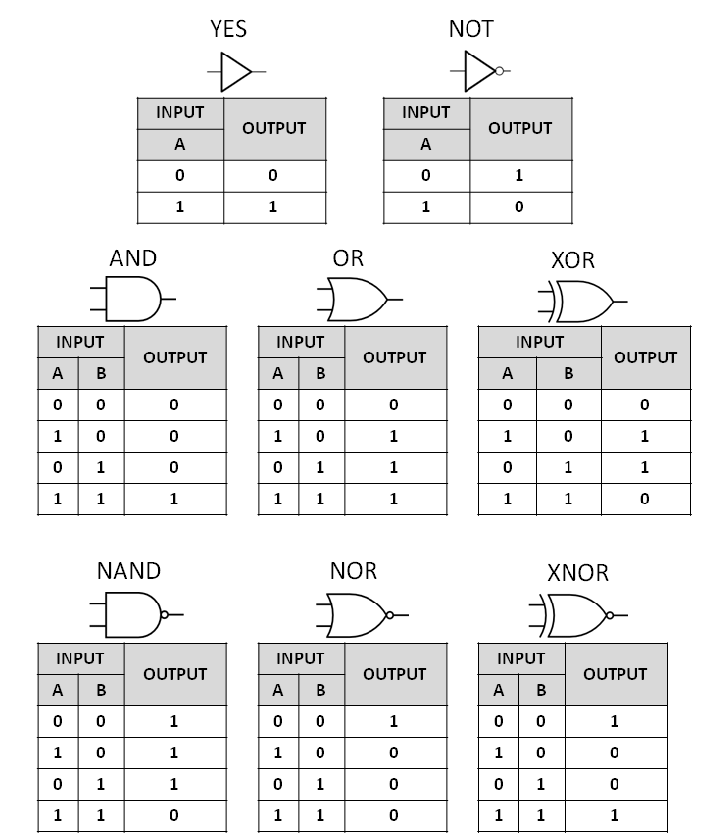
\includegraphics[width=3.6in]{./images/logicGates.png}
        \caption{The common Boolean logic gates with symbols and truth tables}
    \end{figure}
    
    % \item First, remind that sigmoid function looks like figure \ref{fig:RemindSigmoid}.
    \begin{figure}[H]\label{fig:RemindSigmoid}
        \centering
        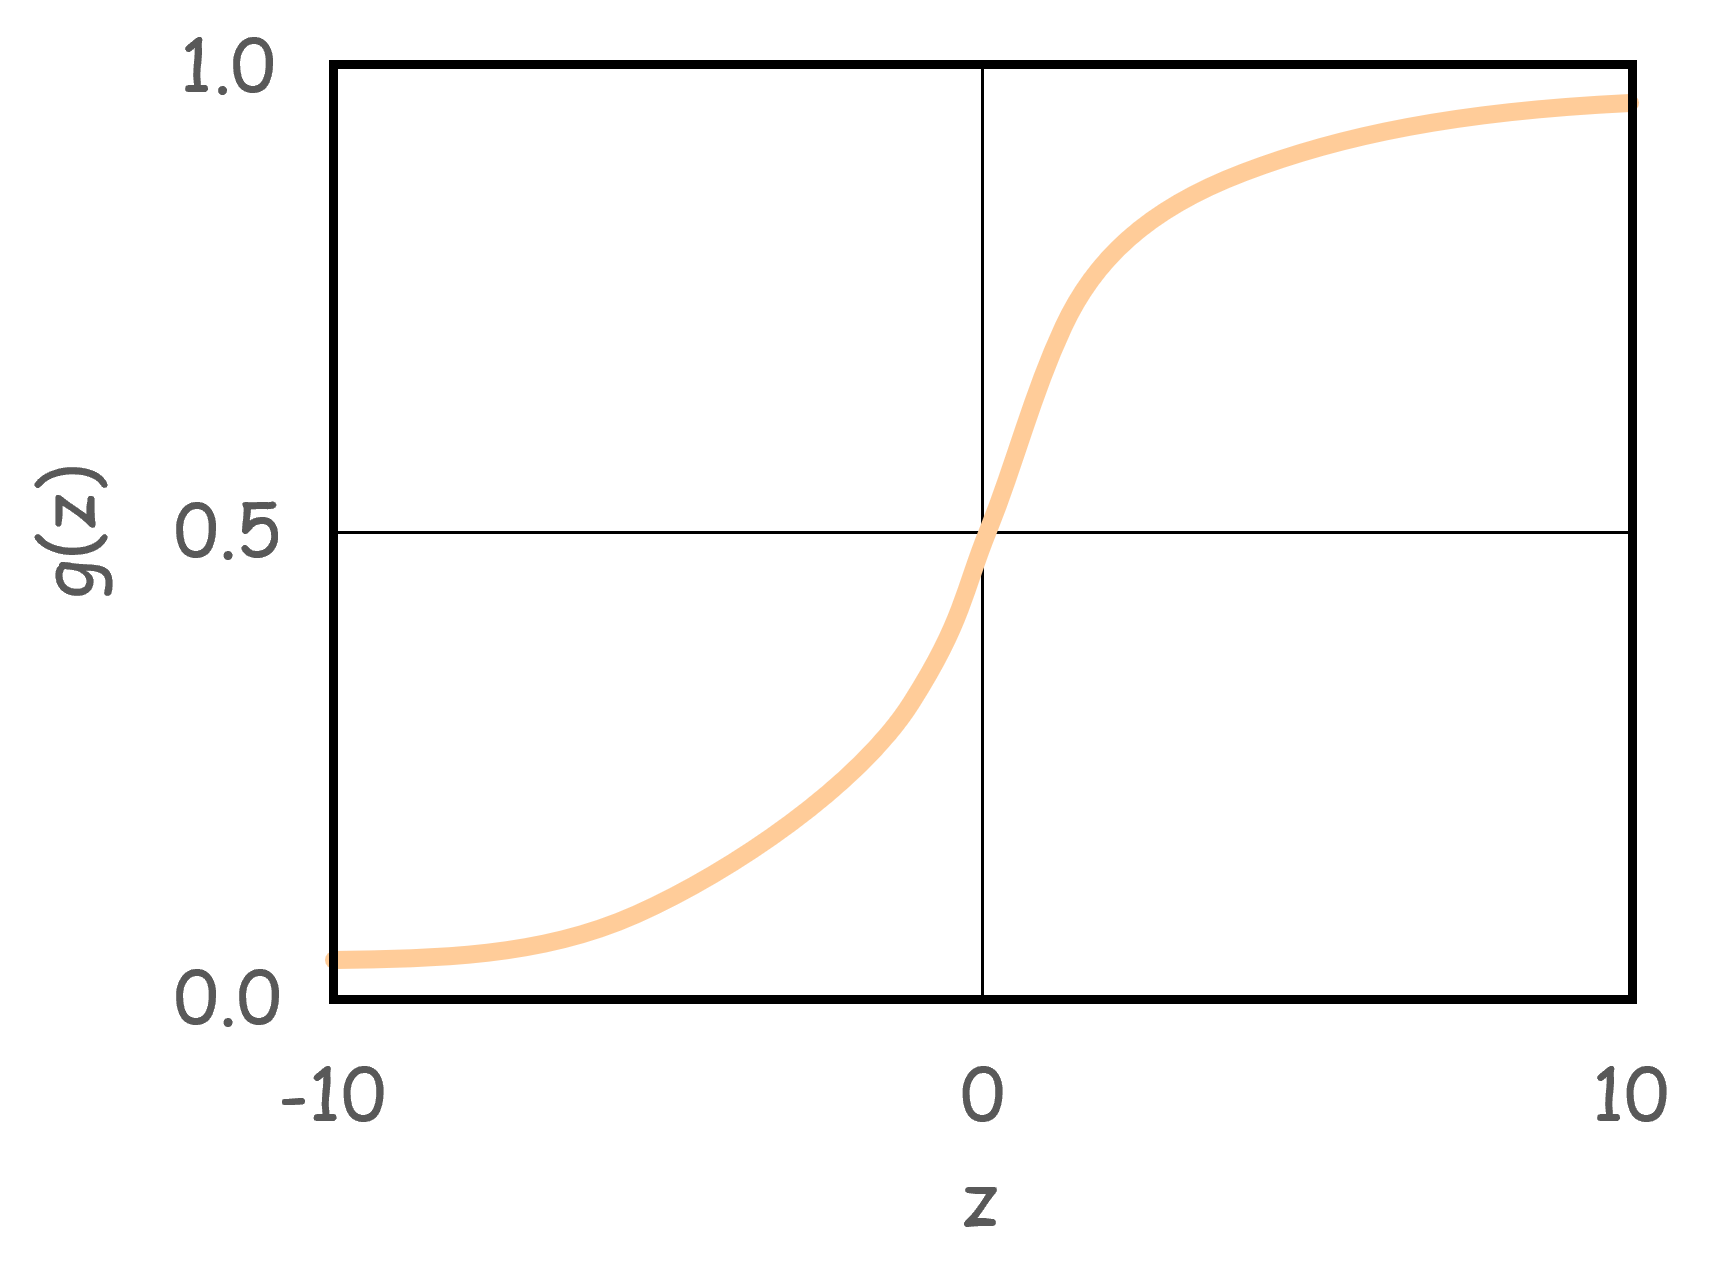
\includegraphics[width=2.8in]{./images/sigmoid.png}
        \caption{Logistic function}
    \end{figure}
    
    \begin{figure}[H]
        \centering
        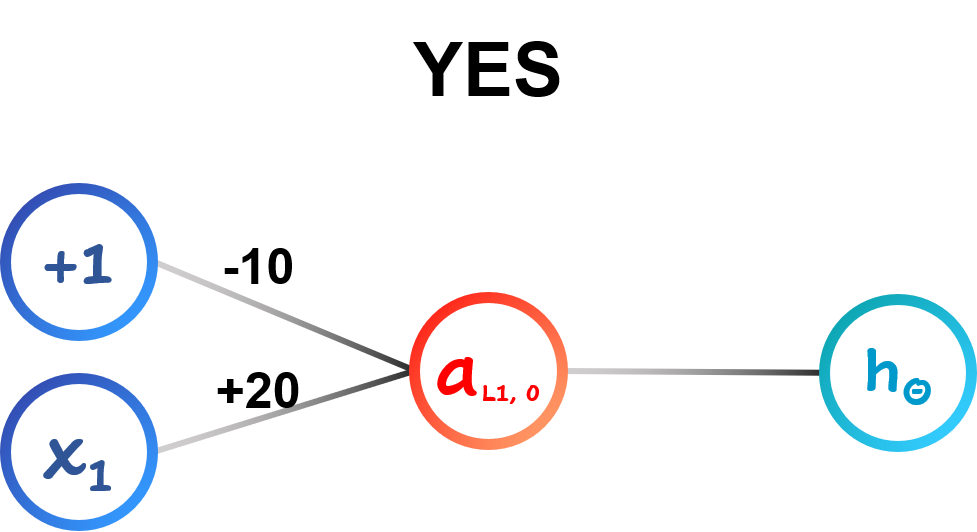
\includegraphics[width=2.4in]{./images/logicGate_YES.png}
        \caption{neural network of logical function YES}
    \end{figure}

    \begin{table}[H]
        \renewcommand\arraystretch{1.5}
        \caption{YES calculation}
        \centering
        \begin{tabular}{ccc}
            \hline\hline %%%%%%%%%%%%%%%%%%%%%%%%%%%%%%%%%%%%%%%%%%%%%%%%%%%%%%%%%%%%%%%%%%%%%%%%%%%%
            Inputs                                                 & Activations        & Outputs    \\ 
            $\begin{array}{ccc} x_0 & x_1 \end{array}$             & $a^{(1)}_0$        & $h$        \\ 
            \hline %%%%%%%%%%%%%%%%%%%%%%%%%%%%%%%%%%%%%%%%%%%%%%%%%%%%%%%%%%%%%%%%%%%%%%%%%%%%%%%%%%
            $\left[{\begin{array}{ccc} 1 & 0 \end{array}}\right]$  & $g(-10) \approx 0$ & $0$        \\
            $\left[{\begin{array}{ccc} 1 & 1 \end{array}}\right]$  & $g(+10) \approx 1$ & $1$        \\[1ex]
            \hline\hline %%%%%%%%%%%%%%%%%%%%%%%%%%%%%%%%%%%%%%%%%%%%%%%%%%%%%%%%%%%%%%%%%%%%%%%%%%%%
        \end{tabular}
    \end{table}
    
    \begin{figure}[H]
        \centering
        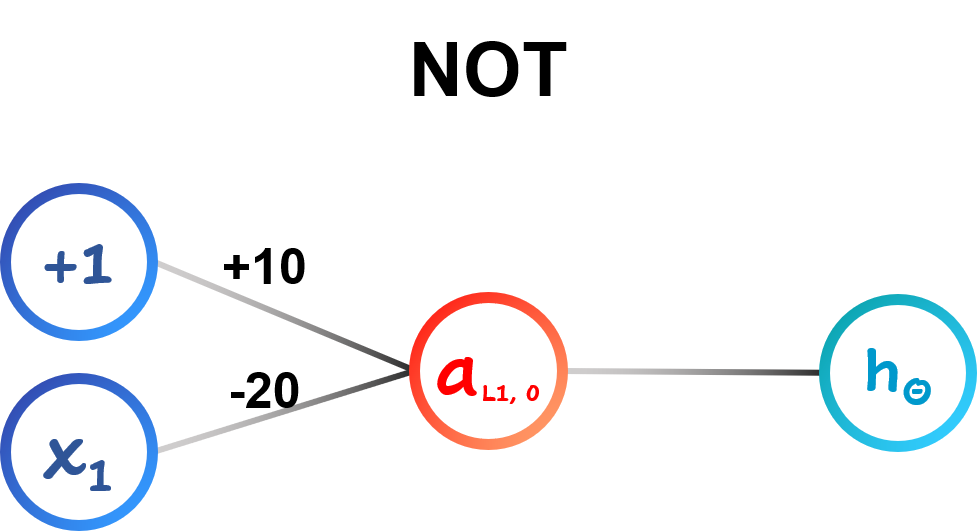
\includegraphics[width=2.4in]{./images/logicGate_NOT.png}
        \caption{neural network of logical function NOT}
    \end{figure}

    \begin{table}[H]
        \renewcommand\arraystretch{1.5}
        \caption{NOT calculation}
        \centering
        \begin{tabular}{ccc}
            \hline\hline %%%%%%%%%%%%%%%%%%%%%%%%%%%%%%%%%%%%%%%%%%%%%%%%%%%%%%%%%%%%%%%%%%%%%%%%%%%%
            Inputs                                                 & Activations        & Outputs    \\ 
            $\begin{array}{ccc} x_0 & x_1 \end{array}$             & $a^{(1)}_0$        & $h$        \\ 
            \hline %%%%%%%%%%%%%%%%%%%%%%%%%%%%%%%%%%%%%%%%%%%%%%%%%%%%%%%%%%%%%%%%%%%%%%%%%%%%%%%%%%
            $\left[{\begin{array}{ccc} 1 & 0 \end{array}}\right]$  & $g(+10) \approx 1$ & $1$        \\
            $\left[{\begin{array}{ccc} 1 & 1 \end{array}}\right]$  & $g(-10) \approx 0$ & $0$        \\[1ex]
            \hline\hline %%%%%%%%%%%%%%%%%%%%%%%%%%%%%%%%%%%%%%%%%%%%%%%%%%%%%%%%%%%%%%%%%%%%%%%%%%%%
        \end{tabular}
    \end{table}
    
    \begin{figure}[H]
        \centering
        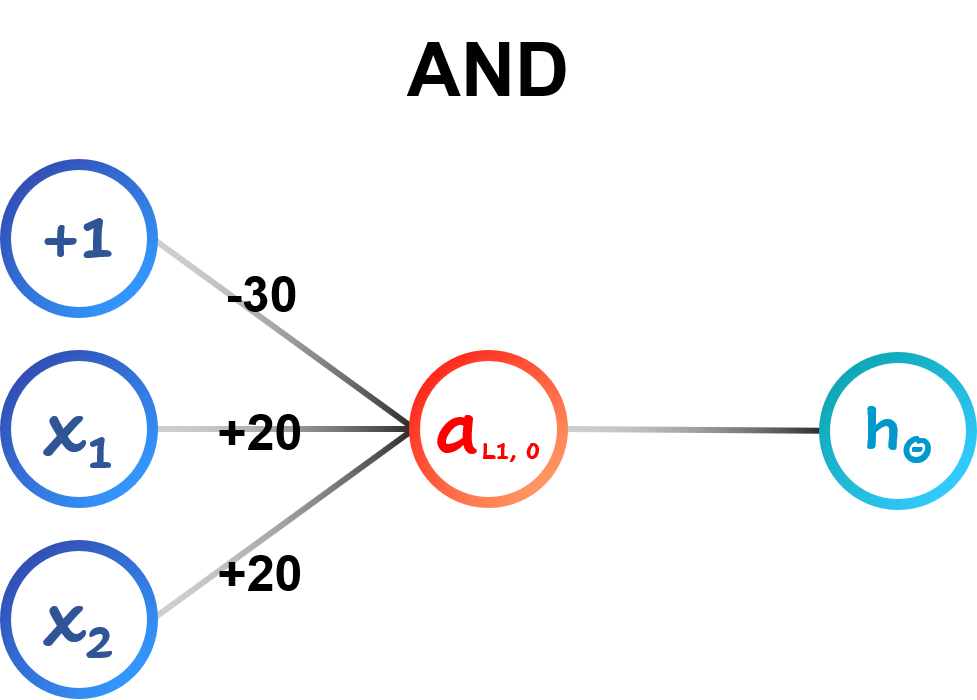
\includegraphics[width=2.4in]{./images/logicGate_AND.png}
        \caption{neural network of logical function AND}
    \end{figure}

    \begin{table}[H]
        \renewcommand\arraystretch{1.5}
        \caption{AND calculation}
        \centering
        \begin{tabular}{ccc}
            \hline\hline %%%%%%%%%%%%%%%%%%%%%%%%%%%%%%%%%%%%%%%%%%%%%%%%%%%%%%%%%%%%%%%%%%%%%%%%%%%%%%%%%%
            Inputs                                                     & Activations        & Outputs    \\ 
            $\begin{array}{ccc} x_0 & x_1 & x_2 \end{array}$           & $a^{(1)}_0$        & $h$        \\ 
            \hline %%%%%%%%%%%%%%%%%%%%%%%%%%%%%%%%%%%%%%%%%%%%%%%%%%%%%%%%%%%%%%%%%%%%%%%%%%%%%%%%%%%%%%%%
            $\left[{\begin{array}{ccc} 1 & 0 & 0 \end{array}}\right]$  & $g(-30) \approx 0$ & $0$        \\ 
            $\left[{\begin{array}{ccc} 1 & 0 & 1 \end{array}}\right]$  & $g(-10) \approx 0$ & $0$        \\
            $\left[{\begin{array}{ccc} 1 & 1 & 0 \end{array}}\right]$  & $g(-10) \approx 0$ & $0$        \\
            $\left[{\begin{array}{ccc} 1 & 1 & 1 \end{array}}\right]$  & $g(+10) \approx 1$ & $1$        \\[1ex]
            \hline\hline %%%%%%%%%%%%%%%%%%%%%%%%%%%%%%%%%%%%%%%%%%%%%%%%%%%%%%%%%%%%%%%%%%%%%%%%%%%%%%%%%%
        \end{tabular}
    \end{table}

    \begin{figure}[H]
        \centering
        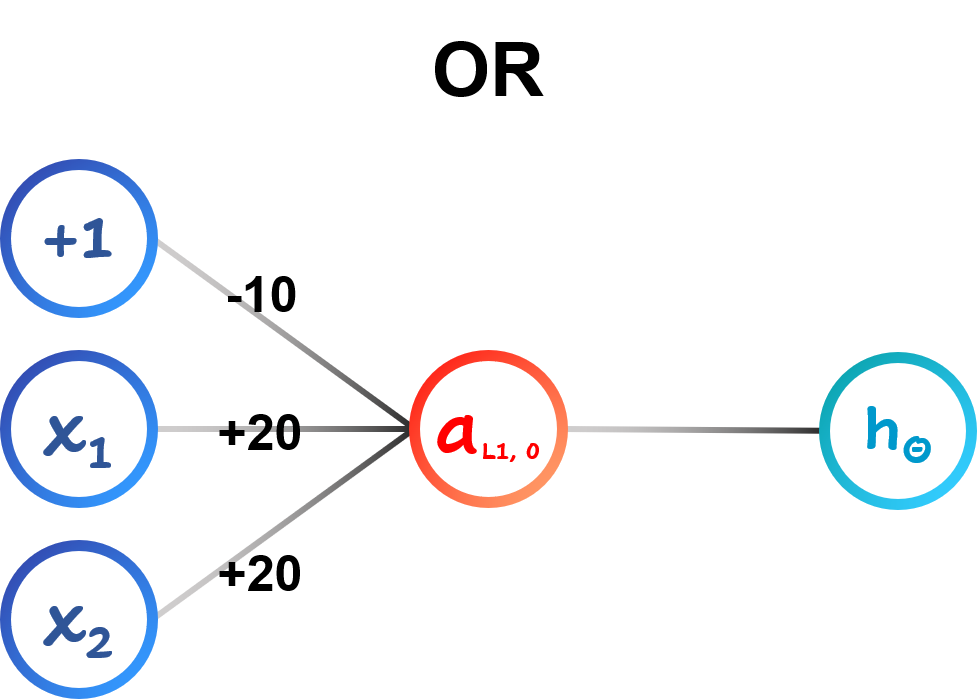
\includegraphics[width=2.4in]{./images/logicGate_OR.png}
        \caption{neural network of logical function OR}
    \end{figure}

    \begin{table}[H]
        \renewcommand\arraystretch{1.5}
        \caption{OR calculation}
        \centering
        \begin{tabular}{ccc}
            \hline\hline %%%%%%%%%%%%%%%%%%%%%%%%%%%%%%%%%%%%%%%%%%%%%%%%%%%%%%%%%%%%%%%%%%%%%%%%%%%%%%%%%%
            Inputs                                                     & Activations        & Outputs    \\ 
            $\begin{array}{ccc} x_0 & x_1 & x_2 \end{array}$           & $a^{(1)}_0$        & $h$        \\ 
            \hline %%%%%%%%%%%%%%%%%%%%%%%%%%%%%%%%%%%%%%%%%%%%%%%%%%%%%%%%%%%%%%%%%%%%%%%%%%%%%%%%%%%%%%%%
            $\left[{\begin{array}{ccc} 1 & 0 & 0 \end{array}}\right]$  & $g(-10) \approx 0$ & $0$        \\ 
            $\left[{\begin{array}{ccc} 1 & 0 & 1 \end{array}}\right]$  & $g(+10) \approx 1$ & $1$        \\
            $\left[{\begin{array}{ccc} 1 & 1 & 0 \end{array}}\right]$  & $g(+10) \approx 1$ & $1$        \\
            $\left[{\begin{array}{ccc} 1 & 1 & 1 \end{array}}\right]$  & $g(+30) \approx 1$ & $1$        \\[1ex]
            \hline\hline %%%%%%%%%%%%%%%%%%%%%%%%%%%%%%%%%%%%%%%%%%%%%%%%%%%%%%%%%%%%%%%%%%%%%%%%%%%%%%%%%%
        \end{tabular}
    \end{table}
    
    \begin{figure}[H]
        \centering
        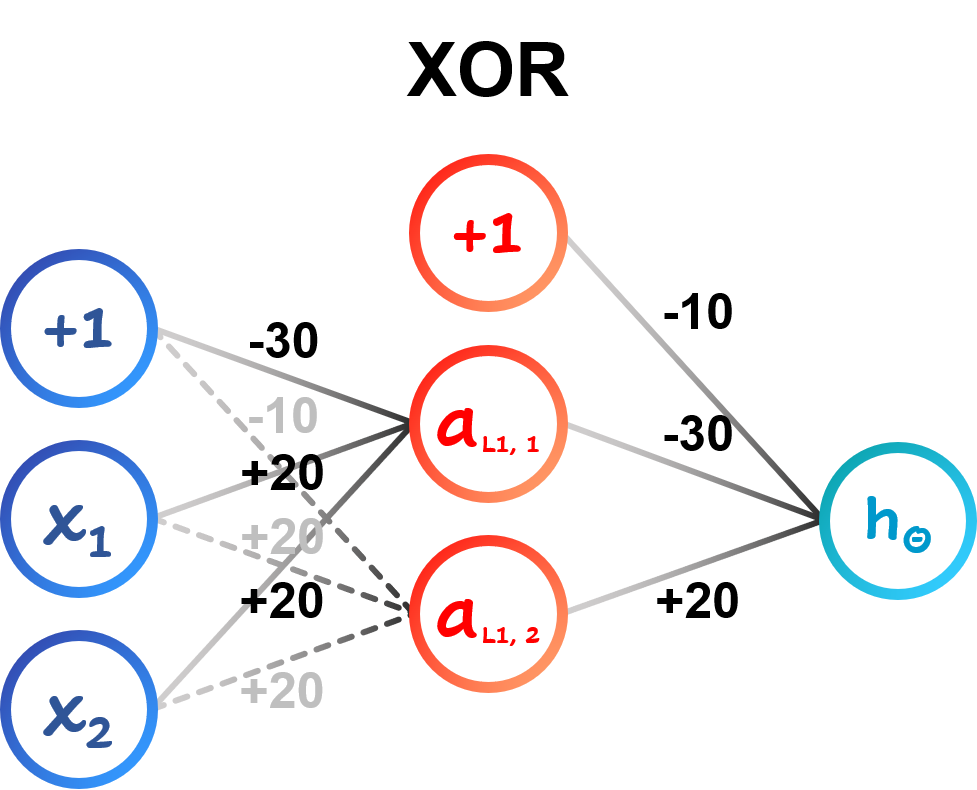
\includegraphics[width=2.4in]{./images/logicGate_XOR.png}
        \caption{neural network of logical function XOR}
    \end{figure}
    
    \begin{table}[H]
        \renewcommand\arraystretch{1.5}
        \caption{XOR calculation}
        \centering
        \begin{tabular}{ccc}
            \hline\hline %%%%%%%%%%%%%%%%%%%%%%%%%%%%%%%%%%%%%%%%%%%%%%%%%%%%%%%%%%%%%%%%%%%%%%%%%%%%%%%%%%%%%%%%%%%%%%%%%%%%%%%%%%%%%%%%%%%%%%%%%%%%%%%%%%%%%%%%%%%%%%%%%%%%%%%%%%%%%%%%%%%%%%%%%%%%%%%%%%%%%%%%%%%%%%%%%%%%%%%%%%%
            Inputs                                                     & Activations                                                                                                                         & Outputs            \\ 
            $\begin{array}{ccc} x_0 & x_1 & x_2 \end{array}$           & $\begin{array}{ccc} a^{(1)}_0 & a^{(1)}_1 & a^{(1)}_2 \end{array}$                                                                  & $h$                \\ 
            \hline %%%%%%%%%%%%%%%%%%%%%%%%%%%%%%%%%%%%%%%%%%%%%%%%%%%%%%%%%%%%%%%%%%%%%%%%%%%%%%%%%%%%%%%%%%%%%%%%%%%%%%%%%%%%%%%%%%%%%%%%%%%%%%%%%%%%%%%%%%%%%%%%%%%%%%%%%%%%%%%%%%%%%%%%%%%%%%%%%%%%%%%%%%%%%%%%%%%%%%%%%%%%%%%%%
            $\left[{\begin{array}{ccc} 1 & 0 & 0 \end{array}}\right]$  & $\left[{\begin{array}{ccc} 1 & g(-30) & g(-10) \end{array}}\right] \approx \left[{\begin{array}{ccc} 1 & 0 & 0 \end{array}}\right]$ & $g(-10) \approx 0$ \\ 
            $\left[{\begin{array}{ccc} 1 & 0 & 1 \end{array}}\right]$  & $\left[{\begin{array}{ccc} 1 & g(-10) & g(+10) \end{array}}\right] \approx \left[{\begin{array}{ccc} 1 & 0 & 1 \end{array}}\right]$ & $g(+10) \approx 1$ \\
            $\left[{\begin{array}{ccc} 1 & 1 & 0 \end{array}}\right]$  & $\left[{\begin{array}{ccc} 1 & g(-10) & g(+10) \end{array}}\right] \approx \left[{\begin{array}{ccc} 1 & 0 & 1 \end{array}}\right]$ & $g(+10) \approx 1$ \\
            $\left[{\begin{array}{ccc} 1 & 1 & 1 \end{array}}\right]$  & $\left[{\begin{array}{ccc} 1 & g(+10) & g(+30) \end{array}}\right] \approx \left[{\begin{array}{ccc} 1 & 1 & 1 \end{array}}\right]$ & $g(-10) \approx 0$ \\[1ex]
            \hline\hline %%%%%%%%%%%%%%%%%%%%%%%%%%%%%%%%%%%%%%%%%%%%%%%%%%%%%%%%%%%%%%%%%%%%%%%%%%%%%%%%%%%%%%%%%%%%%%%%%%%%%%%%%%%%%%%%%%%%%%%%%%%%%%%%%%%%%%%%%%%%%%%%%%%%%%%%%%%%%%%%%%%%%%%%%%%%%%%%%%%%%%%%%%%%%%%%%%%%%%%%%%%
        \end{tabular}
    \end{table}

    \begin{figure}[H]
        \centering
        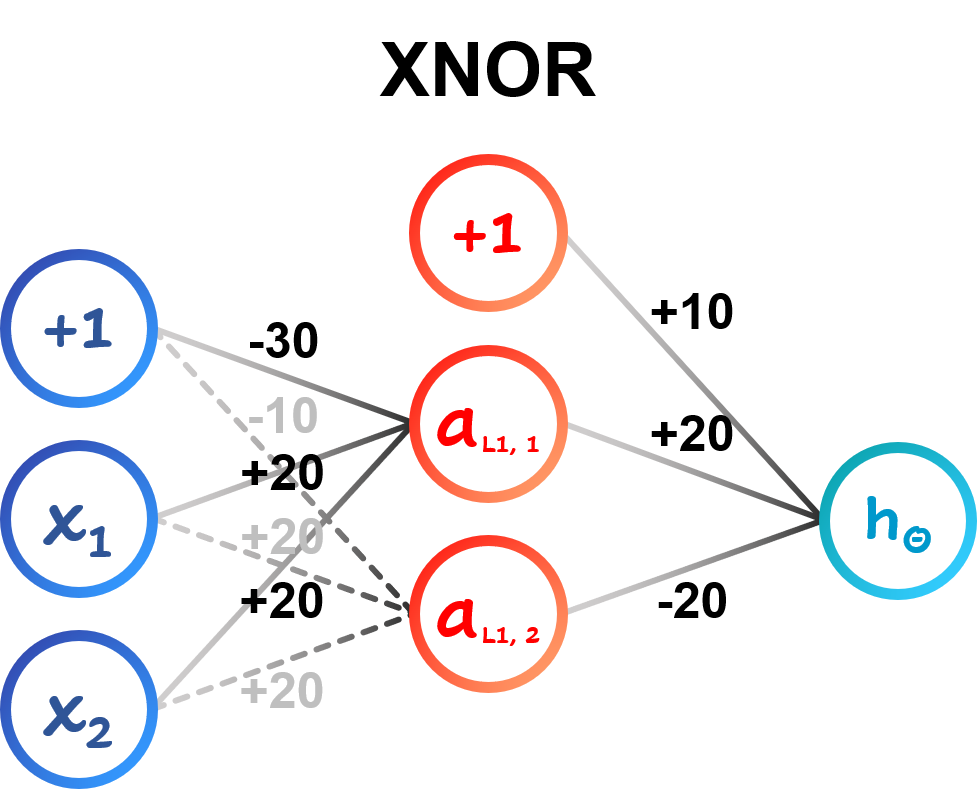
\includegraphics[width=2.4in]{./images/logicGate_XNOR.png}
        \caption{neural network of logical function XNOR}
    \end{figure}
    
    \begin{table}[H]
        \renewcommand\arraystretch{1.5}
        \caption{XNOR calculation}
        \centering
        \begin{tabular}{ccc}
            \hline\hline %%%%%%%%%%%%%%%%%%%%%%%%%%%%%%%%%%%%%%%%%%%%%%%%%%%%%%%%%%%%%%%%%%%%%%%%%%%%%%%%%%%%%%%%%%%%%%%%%%%%%%%%%%%%%%%%%%%%%%%%%%%%%%%%%%%%%%%%%%%%%%%%%%%%%%%%%%%%%%%%%%%%%%%%%%%%%%%%%%%%%%%%%%%%%%%%%%%%%%%%%%%
            Inputs                                                     & Activations                                                                                                                         & Outputs            \\ 
            $\begin{array}{ccc} x_0 & x_1 & x_2 \end{array}$           & $\begin{array}{ccc} a^{(1)}_0 & a^{(1)}_1 & a^{(1)}_2 \end{array}$                                                                  & $h$                \\ 
            \hline %%%%%%%%%%%%%%%%%%%%%%%%%%%%%%%%%%%%%%%%%%%%%%%%%%%%%%%%%%%%%%%%%%%%%%%%%%%%%%%%%%%%%%%%%%%%%%%%%%%%%%%%%%%%%%%%%%%%%%%%%%%%%%%%%%%%%%%%%%%%%%%%%%%%%%%%%%%%%%%%%%%%%%%%%%%%%%%%%%%%%%%%%%%%%%%%%%%%%%%%%%%%%%%%%
            $\left[{\begin{array}{ccc} 1 & 0 & 0 \end{array}}\right]$  & $\left[{\begin{array}{ccc} 1 & g(-30) & g(-10) \end{array}}\right] \approx \left[{\begin{array}{ccc} 1 & 0 & 0 \end{array}}\right]$ & $g(+10) \approx 1$ \\ 
            $\left[{\begin{array}{ccc} 1 & 0 & 1 \end{array}}\right]$  & $\left[{\begin{array}{ccc} 1 & g(-10) & g(+10) \end{array}}\right] \approx \left[{\begin{array}{ccc} 1 & 0 & 1 \end{array}}\right]$ & $g(-10) \approx 0$ \\
            $\left[{\begin{array}{ccc} 1 & 1 & 0 \end{array}}\right]$  & $\left[{\begin{array}{ccc} 1 & g(-10) & g(+10) \end{array}}\right] \approx \left[{\begin{array}{ccc} 1 & 0 & 1 \end{array}}\right]$ & $g(-10) \approx 0$ \\
            $\left[{\begin{array}{ccc} 1 & 1 & 1 \end{array}}\right]$  & $\left[{\begin{array}{ccc} 1 & g(+10) & g(+30) \end{array}}\right] \approx \left[{\begin{array}{ccc} 1 & 1 & 1 \end{array}}\right]$ & $g(+10) \approx 1$ \\[1ex]
            \hline\hline %%%%%%%%%%%%%%%%%%%%%%%%%%%%%%%%%%%%%%%%%%%%%%%%%%%%%%%%%%%%%%%%%%%%%%%%%%%%%%%%%%%%%%%%%%%%%%%%%%%%%%%%%%%%%%%%%%%%%%%%%%%%%%%%%%%%%%%%%%%%%%%%%%%%%%%%%%%%%%%%%%%%%%%%%%%%%%%%%%%%%%%%%%%%%%%%%%%%%%%%%%%
        \end{tabular}
    \end{table}    
\end{itemize}
        